\begin{figure}[p]
  \centering
  \subfloat[Main Menu UI]{
    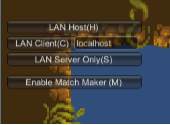
\includegraphics[width=0.3\linewidth]{UNET/Main_Menu_UI}
  }
  \qquad
  \subfloat[Host UI]{
    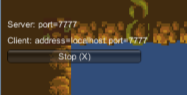
\includegraphics[width=0.3\textwidth]{UNET/Host_UI}
  }
  \qquad
  \subfloat[Client UI]{
    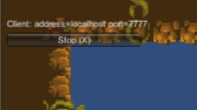
\includegraphics[width=0.3\linewidth]{UNET/Client_UI}
  }

  \caption{UNET default UI}
  \label{fig:unet_ui}
\end{figure}

\begin{figure}[p]
  \centering
  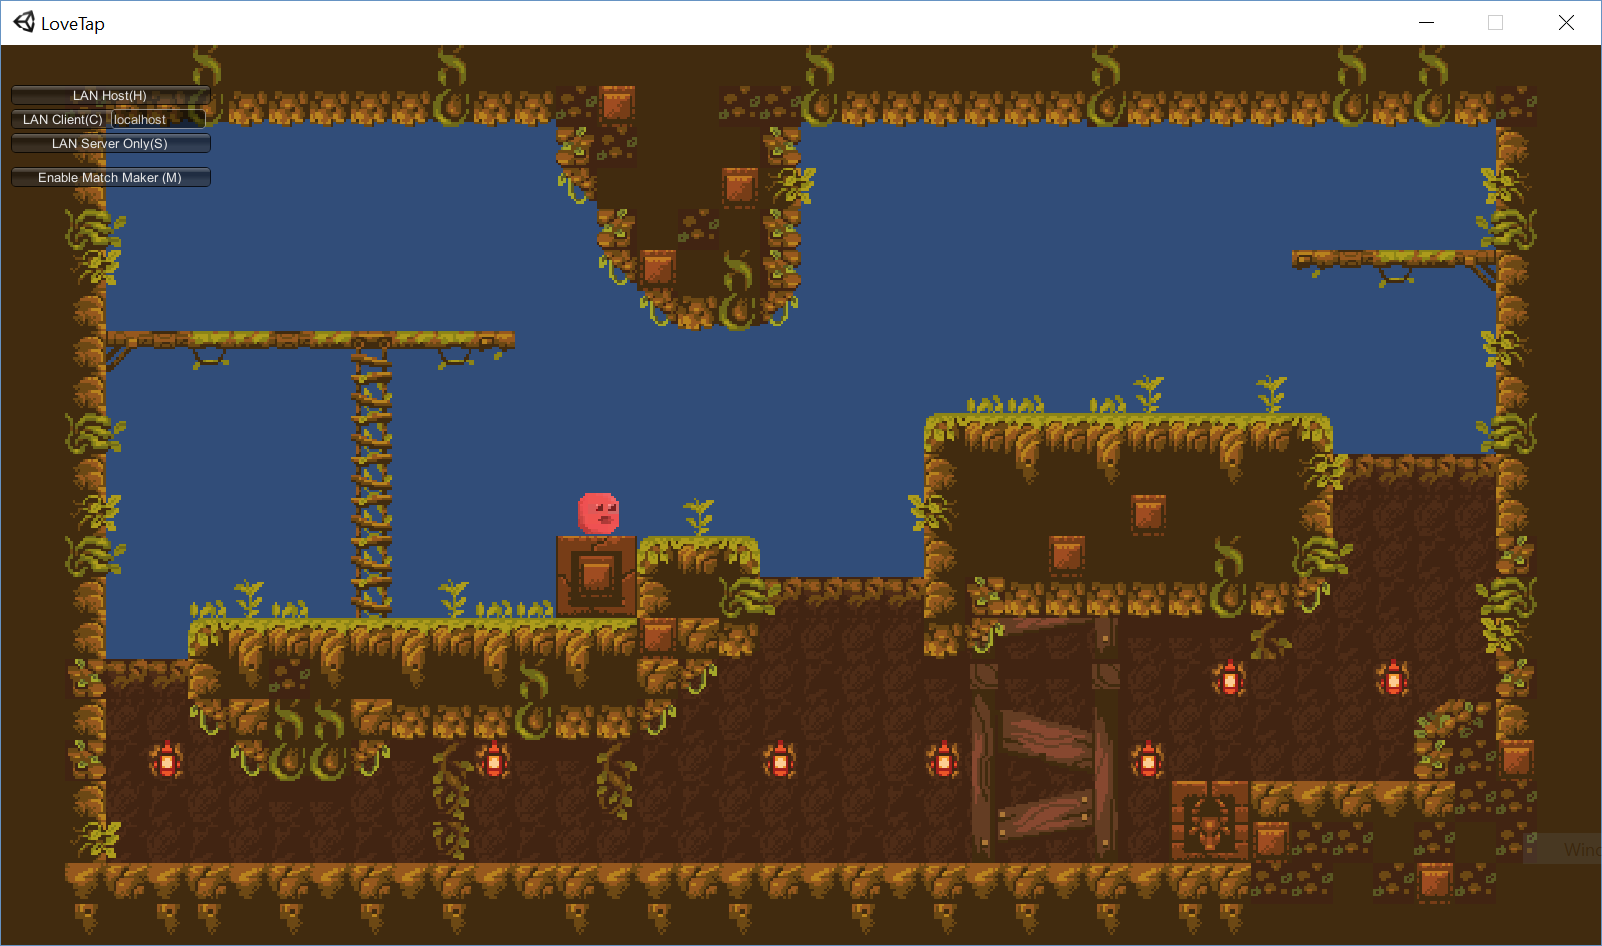
\includegraphics[width=\textwidth]{UNET/Main_Menu}
  \caption{Main Menu}
  \label{fig:main}
\end{figure}


\begin{figure}[p]
  \centering

  \subfloat[Host game screen]{
    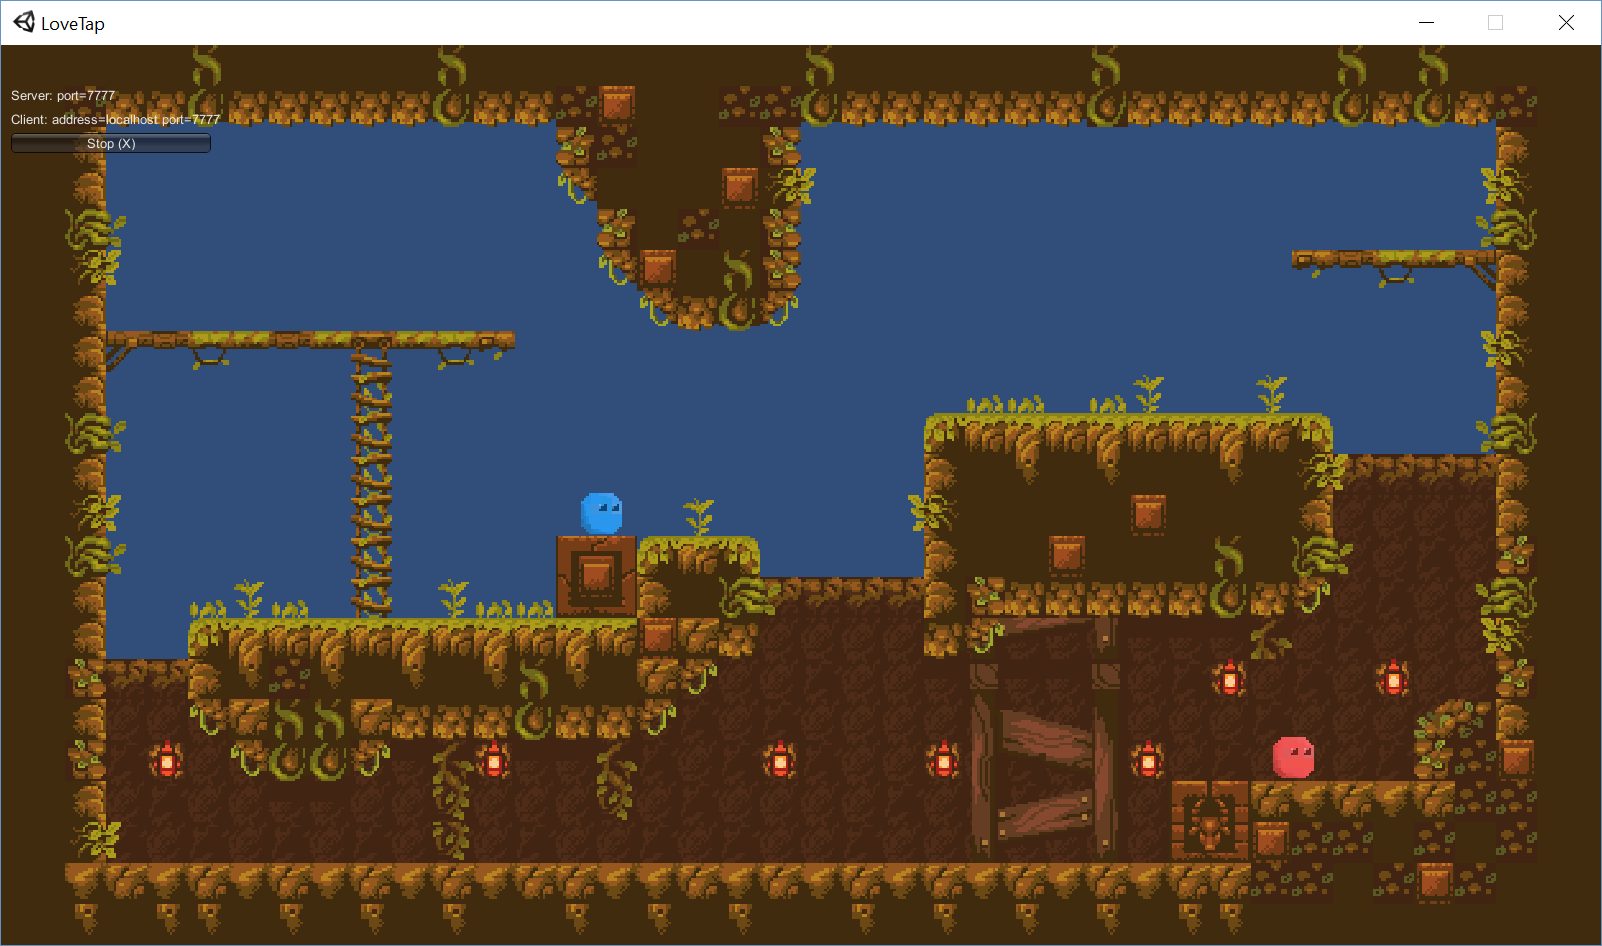
\includegraphics[width=0.45\textwidth]{UNET/Host}
  }
  \qquad
  \subfloat[Client game screen]{
    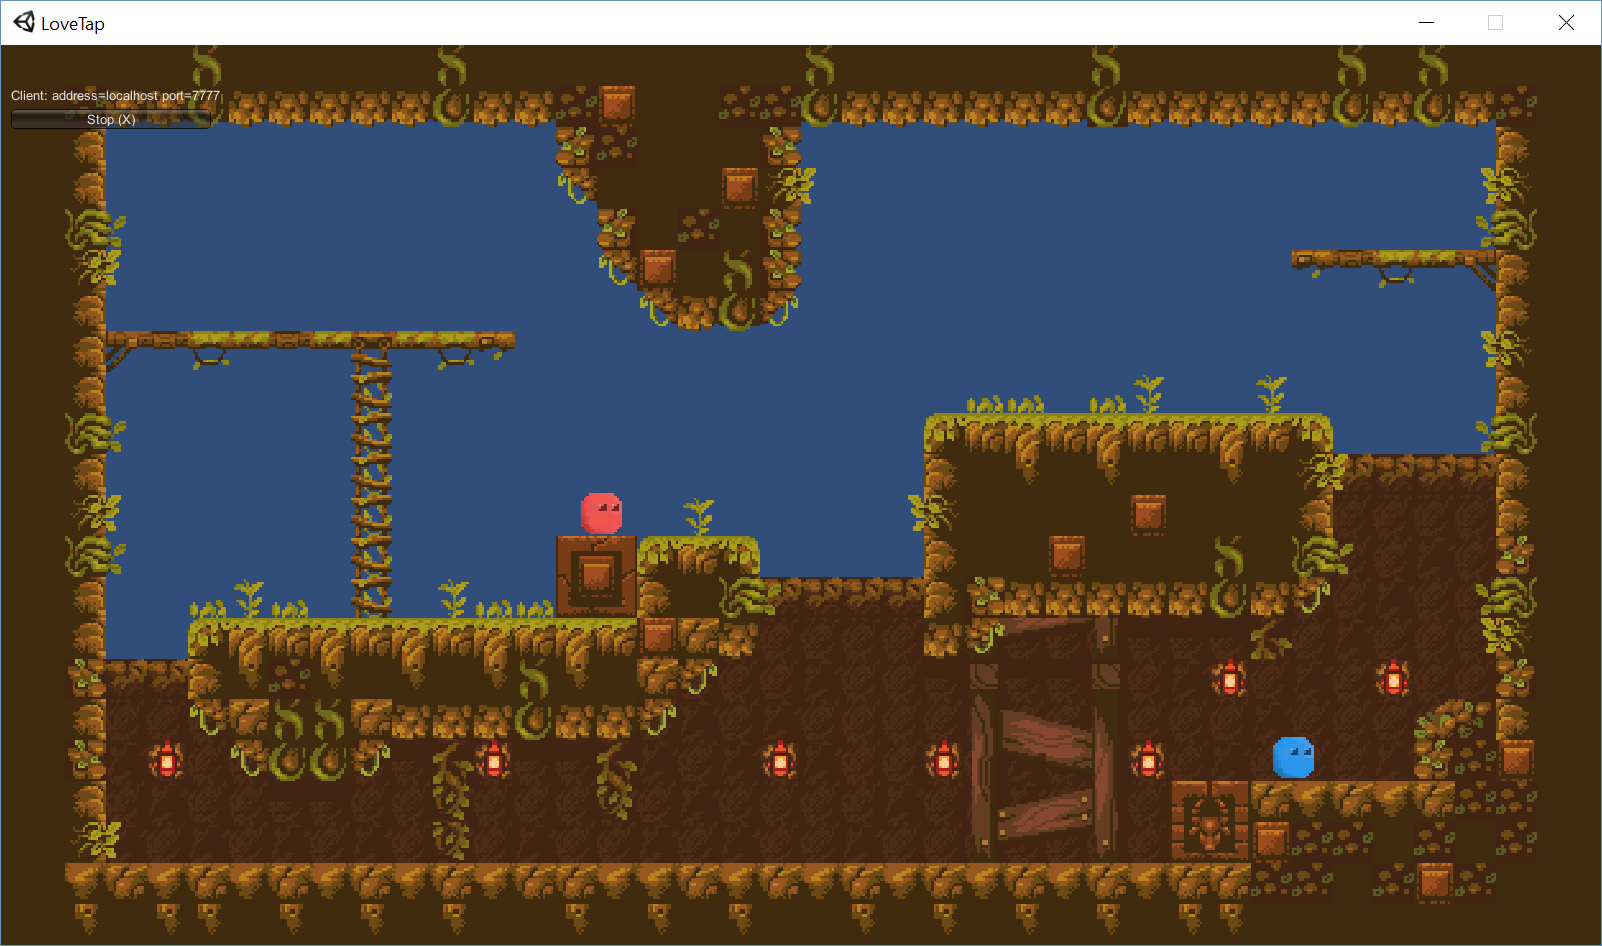
\includegraphics[width=0.45\linewidth]{UNET/Client}
  }

  \caption{Main game loop after connection is established}
  \label{fig:in_game}
\end{figure}
